\subsection{Data Storage and Access}

\begin{frame}{Traditional Inodes}
    \begin{itemize}
        \item used in many file system structures (e.g. ext3)
        \item each node has an index
        \item bijective mapping (file $\leftrightarrow$ inode)
        \item contains \textbf{metadata} and \textbf{data location} (pointer)
    \end{itemize}
\end{frame}

\begin{frame}{Metadata (Lustre Inodes)}
    \begin{itemize}
        \item Lustre uses similar structure
        \item inodes are stored on MDT
        \item inodes point to objects on OSTs
        \item file is \emph{striped} across multiple OSTs
        \item inode stores information to these OSTs
    \end{itemize}
\end{frame}

\begin{frame}{Striping}
    \begin{itemize}
        \item RAID-0 type striping
        \item data is split into blocks
        \item block size adjustable per file/directory
        \item OSTs store every n-th block (with n being number of OSTs involved)
        \item speed advantage (multiple simultaneous OSS/OST connections)
        \item capacity advantage (file bigger than single OST)
    \end{itemize}

    \tikzset{
        block/.style = {rectangle,fill=black!10!white,minimum width=1cm,minimum height=0.3cm,inner sep=0pt,draw=black},
        a/.style = {fill=red!30!white},
        b/.style = {fill=green!30!white},
        ost/.style = {rectangle, rounded corners=3pt, draw=black!30!white, thick, fill=black!5!white, minimum width=1.6cm, minimum height=2cm},
        object/.style = {rectangle, draw=black!50!white, very thick, minimum width=1cm}
    }

    \vspace{0.2cm}
    \makebox[\textwidth][c] {
        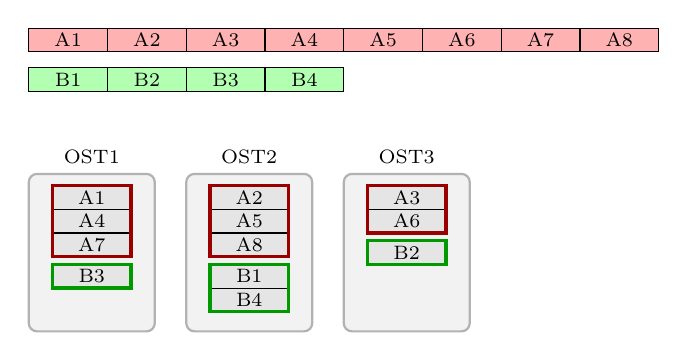
\begin{tikzpicture}[x=1cm,y=1cm,every node/.style={font=\scriptsize}]
            \node[block,a] (a1) at (0.5, -0.3) {A1};
            \node[block,a] (a2) at (1.5, -0.3) {A2};
            \node[block,a] (a3) at (2.5, -0.3) {A3};
            \node[block,a] (a4) at (3.5, -0.3) {A4};
            \node[block,a] (a5) at (4.5, -0.3) {A5};
            \node[block,a] (a6) at (5.5, -0.3) {A6};
            \node[block,a] (a7) at (6.5, -0.3) {A7};
            \node[block,a] (a8) at (7.5, -0.3) {A8};

            \node[block,b] (b1) at (0.5, -0.8) {B1};
            \node[block,b] (b2) at (1.5, -0.8) {B2};
            \node[block,b] (b3) at (2.5, -0.8) {B3};
            \node[block,b] (b4) at (3.5, -0.8) {B4};

            \node[ost,label=above:OST1] (ost1) at (0.8, -3) {};
            \node[ost,label=above:OST2] (ost1) at (2.8, -3) {};
            \node[ost,label=above:OST3] (ost1) at (4.8, -3) {};

            \node[block] (da1) at (0.8, -2.3) {A1};
            \node[block] (da2) at (2.8, -2.3) {A2};
            \node[block] (da3) at (4.8, -2.3) {A3};
            \node[block] (da4) at (0.8, -2.6) {A4};
            \node[block] (da5) at (2.8, -2.6) {A5};
            \node[block] (da6) at (4.8, -2.6) {A6};
            \node[block] (da7) at (0.8, -2.9) {A7};
            \node[block] (da8) at (2.8, -2.9) {A8};

            \node[block] (db1) at (2.8, -3.3) {B1};
            \node[block] (db2) at (4.8, -3.0) {B2};
            \node[block] (db3) at (0.8, -3.3) {B3};
            \node[block] (db4) at (2.8, -3.6) {B4};

            \node[object,minimum height=0.9cm,draw=red!60!black] (o1) at (0.8, -2.6) {};
            \node[object,minimum height=0.9cm,draw=red!60!black] (o2) at (2.8, -2.6) {};
            \node[object,minimum height=0.6cm,draw=red!60!black] (o3) at (4.8, -2.45) {};

            \node[object,minimum height=0.6cm,draw=green!60!black] (o4) at (2.8, -3.45) {};
            \node[object,minimum height=0.3cm,draw=green!60!black] (o4) at (0.8, -3.3) {};
            \node[object,minimum height=0.3cm,draw=green!60!black] (o4) at (4.8, -3.0) {};
        \end{tikzpicture}
    }
\end{frame}

\begin{frame}{Data Safety \& Integrity}
    \begin{itemize}
        \item data safety
            \begin{itemize}
                \item striping does \textbf{not} backup any data
                \item \emph{but} for the targets, a RAID can be used
                \item in target RAIDs, a drive may fail (depends on RAID type)
            \end{itemize}
        \item availability
            \begin{itemize}
                \item failovers ensure target reachability
                \item multiple network types/connections
            \end{itemize}
        \item consistency
            \begin{itemize}
                \item lustre log (similar to journal)
                \item simultaneous write protection: LDLM (Lustre Distributed Lock Manager),
                    distributed across OSS
            \end{itemize}
    \end{itemize}
\end{frame}
